% Created 2013-04-26 Ven 08:18
\documentclass[bigger,hyperref={colorlinks=true, urlcolor=red, plainpages=false, pdfpagelabels, bookmarksnumbered}]{beamer}
\usepackage[utf8]{inputenc}
\usepackage[T1]{fontenc}
\usepackage{fixltx2e}
\usepackage{graphicx}
\usepackage{longtable}
\usepackage{float}
\usepackage{wrapfig}
\usepackage{soul}
\usepackage{textcomp}
\usepackage{marvosym}
\usepackage{wasysym}
\usepackage{latexsym}
\usepackage{amssymb}
\usepackage{hyperref}
\tolerance=1000
\usepackage{color}
\usepackage{listings}
\AtBeginSection[]{\begin{frame}<beamer>\frametitle{Table of Contents}\tableofcontents[currentsection]\end{frame}}
\lstset{
keywordstyle=\color{blue},
commentstyle=\color{red},
stringstyle=\color{green},
basicstyle=\ttfamily\footnotesize,
columns=fullflexible,
frame=single,
basewidth={0.5em,0.4em}
}
\RequirePackage{fancyvrb}
\DefineVerbatimEnvironment{verbatim}{Verbatim}{fontsize=\small,formatcom = {\color[rgb]{0.5,0,0}}}
\providecommand{\alert}[1]{\textbf{#1}}

\title{Introduction to Cloud Computing}
\author{Stephane Genaud}
\date{\today}
\hypersetup{
  pdfkeywords={},
  pdfsubject={},
  pdfcreator={Emacs Org-mode version 7.8.11}}

\usetheme{Boadilla}\usecolortheme{default}
\setbeamertemplate{footline}{\leavevmode \hbox{ \begin{beamercolorbox}[wd=.6\paperwidth,ht=2.25ex,dp=1ex,center]{title in head/foot} \insertshorttitle\end{beamercolorbox} \begin{beamercolorbox}[wd=.25\paperwidth,ht=2.25ex,dp=1ex,center]{date in head/foot}\insertshortauthor\end{beamercolorbox} \begin{beamercolorbox}[wd=.15\paperwidth,ht=2.25ex,dp=1ex,right]{title in head/foot} \insertframenumber / \inserttotalframenumber\hspace*{2em} \end{beamercolorbox} } \vskip0pt }
\setbeamercovered{invisible}
\author[S. Genaud]{{\large Stéphane Genaud} \\ \vspace{0.2cm} ENSIIE - Strasbourg \\ \vspace{0.2cm} \texttt{genaud@ensiie.fr} }
\date{{\large Introduction to Cloud Computing} \\ \vspace{0.2cm} }
\begin{document}

\maketitle

\begin{frame}
\frametitle{Outline}
\setcounter{tocdepth}{3}
\tableofcontents
\end{frame}





\section{Introduction}
\label{sec-1}
\begin{frame}
\frametitle{Today: Distributed Services are everywhere}
\label{sec-1-1}
\begin{block}{Storage and Computing}
\label{sec-1-1-1}

   
\includegraphics[width=.25\textwidth]{img/logo_evernote.png}
   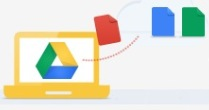
\includegraphics[width=.19\textwidth]{img/logo_google_doc.jpg}
   
\includegraphics[width=.12\textwidth]{img/logo_google_maps.png}


   
\includegraphics[width=.25\textwidth]{img/logo_dropbox.png}
   
\includegraphics[width=.25\textwidth]{img/logo_picasa.png}
\end{block}
\end{frame}
\begin{frame}
\frametitle{Technologies for Distributed Systems}
\label{sec-1-2}

\begin{itemize}
\item Extremely fast evolution of DS since 1985.
\item Distributed System design adapts to hardware technology evolution.
\end{itemize}
\end{frame}
\begin{frame}
\frametitle{A Time-line of technologies}
\label{sec-1-3}

  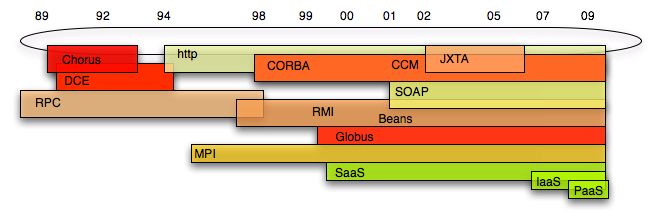
\includegraphics[width=.8\linewidth]{../img/timeline.png}
\end{frame}
\begin{frame}
\frametitle{Cloud Computing}
\label{sec-1-4}
\begin{block}{Cloud Computing: A definition}
\label{sec-1-4-1}

    General Definition: The ability to compute or store data at \emph{some} location 
    and retrieve them from ubiquitous and various devices.
  
\end{block}
\begin{itemize}

\item Notes
\label{sec-1-4-2}%
\begin{itemize}
\item Tablets, smartphones, and not only desktops and laptops
\item Note: \emph{Why cloud computing even for data storage?} Maybe because, computations take place near the data.
\end{itemize}

\end{itemize} % ends low level
\end{frame}
\begin{frame}
\frametitle{Enabling Technologies}
\label{sec-1-5}
\begin{block}{Enabling Technologies}
\label{sec-1-5-1}

\begin{itemize}
\item Web 2.0 (REST design)
\item Distributed Storage (originates in P2P file-systems)
\item Virtualization
\item Network bandwidth and latency
\item Asymetric ciphering (RSA, then PGP)
\end{itemize}
      
\end{block}
\end{frame}
\section{Main Characteristics}
\label{sec-2}
\begin{frame}
\frametitle{Clouds' Characteristics}
\label{sec-2-1}

Cloud Computing can be caracterized by:
\begin{itemize}
\item Types of Services: SaaS, IaaS, PaaS
\item A new business model
\item Elasticity
\end{itemize}
\end{frame}
\begin{frame}
\frametitle{SaaS}
\label{sec-2-2}

\emph{Software as a Service} 
\begin{itemize}
\item users have only access to the service (hosted \emph{somewhere})
\item long standing form of cloud computing (before the name existed)
\item e.g Gmail, Hotmail, Dropbox, \ldots{}
\end{itemize}
\end{frame}
\begin{frame}
\frametitle{IaaS}
\label{sec-2-3}

\emph{Infrastructure as a Service}
\begin{itemize}
\item users are granted a total control over machines they can start/stop
\item machines are totally controlled by the user (e.g through ssh)
\item e.g Amazon EC2 and S3, Google Compute Engine, recently Microsoft Azure
\end{itemize}
\end{frame}
\begin{frame}
\frametitle{PaaS}
\label{sec-2-4}

\emph{Platform as a Service}
\begin{itemize}
\item users are given a library or a framework to develop their applications
\item the application is deployed over a cloud by the provider
\item e.g Google App Engine, Microsoft Azure
\end{itemize}
\end{frame}
\begin{frame}
\frametitle{Business Model}
\label{sec-2-5}
\begin{itemize}

\item Clients
\label{sec-2-5-1}%
\begin{itemize}
\item \emph{pay-as-you-go} model, almost always per-hour
\end{itemize}

\item Provider
\label{sec-2-5-2}%
\begin{itemize}
\item consolidation of VMs onto PMs
\item investment in hardware and software are armotized in large data-centers
      \emph{price in medium (1K-server) data center is 5 to 7 times the one in large datacenters (50K)}
\end{itemize}

\end{itemize} % ends low level
\end{frame}
\begin{frame}
\frametitle{Amazon's EC2 illustration}
\label{sec-2-6}


On-demand instance, Linux, USA-West. Partial list (on 04/25/2013)


\begin{center}
\begin{tabular}{lrlr}
 Instance      &  price (\$/hour)  &  CPU            &  RAM (GB)  \\
\hline
 m1.small      &             0.06  &  1 Vcore        &       1.7  \\
 m1.medium     &             0.12  &  1 Vcore x2     &      3.75  \\
 m1.large      &             0.24  &  2 Vcore x2     &       7.5  \\
 m1.xlarge     &             0.48  &  4 Vcore x2     &        15  \\
\hline
 m2.xlarge     &             0.41  &  4 Vcore x3.25  &      17.1  \\
 m2.2xlarge    &             0.82  &  8 Vcore x3.25  &      34.2  \\
\hline
 c1.medium     &            0.145  &  2 Vcore x2.5   &       1.7  \\
 c1.xlarge     &            0.580  &  8 Vcore x2.5   &         7  \\
\hline
 cc2.8.xlarge  &             2.40  &  2x8Vcore x5.5  &      60.5  \\
\hline
\end{tabular}
\end{center}
\end{frame}
\begin{frame}
\frametitle{Elasticity}
\label{sec-2-7}

\begin{itemize}
\item \emph{pay-as-you-go} model encourages elastic provisioning
\item VM starts in a couple of minutes
\item Manual or automatic scaling (e.g \href{http://www.rightscale.com}{RightSscale})
\end{itemize}
\end{frame}
\section{What are Clouds used for?}
\label{sec-3}
\begin{frame}
\frametitle{Web applications and contents}
\label{sec-3-1}

\begin{itemize}
\item Scalable delivery of contents 
     e.g Amazon CloudFront
\end{itemize}
\end{frame}
\begin{frame}
\frametitle{Data storage}
\label{sec-3-2}

\begin{itemize}
\item Scalable data storage
\item e.g GoogleDrive, Dropbox, iCloud
\item Use of distributed storage systems, generally NoSQL systems
\item e.g Cassandra, Dynamo, CouchDB
\end{itemize}
\end{frame}
\begin{frame}
\frametitle{Analytics}
\label{sec-3-3}

\begin{itemize}
\item Batch jobs for parameter sweep computations
\item Parallel jobs  (e.g Map-Reduce for PageRank)
\end{itemize}
\end{frame}
\section{Support Paper}
\label{sec-4}
\begin{frame}
\frametitle{Above the Clouds: A Berkeley View of Cloud Computing}
\label{sec-4-1}


\begin{itemize}
\item a paper from feb 2009 (Amazon \href{http://aws.typepad.com/aws/2006/08/amazon_ec2_beta.html}{announced} EC2 Beta opening in 2006)
\item defines cloud computing (Section 3)
\item explains the reasons why Cloud Computing succeeds (Section 4)
\item browses the offers of Utility Computing (Section 5)
\item describes the economics behind cloud computing (Section 6)
\item list obstacles and opportunities (Section 7)
\end{itemize}
\end{frame}
\begin{frame}
\frametitle{Concepts}
\label{sec-4-2}
\begin{itemize}

\item DataCenter Economics
\label{sec-4-2-1}%

\item VM -- Virtualization
\label{sec-4-2-2}%

\item Pricing model
\label{sec-4-2-3}%

\item Lock-In and Availability Issues
\label{sec-4-2-4}%

\item Data Storage
\label{sec-4-2-5}%

\item Parallel jobs
\label{sec-4-2-6}%


\end{itemize} % ends low level
\end{frame}

\end{document}
